\documentclass[aspectratio=169]{beamer}

\usetheme{Madrid}
\usecolortheme{default}

\usepackage[utf8]{inputenc}
\usepackage[T1]{fontenc}
\usepackage{amsmath}
\usepackage{booktabs}
\usepackage{tikz}
\usetikzlibrary{arrows.meta, positioning, shapes.geometric, decorations.pathreplacing}

\title[CoopInfer]{CoopInfer: Host--Device Cooperative Inference Scheduling}
\subtitle{A strategy-driven prototype for DAG partitioning and schedule visualization}
\author{CoopInfer Project}
\date{\today}

\newcommand{\device}{\textsc{Device}}
\newcommand{\host}{\textsc{Host}}

\begin{document}

\begin{frame}
  \titlepage
\end{frame}

\begin{frame}{Motivation}
  \begin{itemize}
    \item Embodied AI pipelines often run as DAGs of perception, fusion, and control operators.
    \item Some operators must stay on the robot-side device, while others may run on an edge host.
    \item The scheduling problem is not only graph partitioning:
      \begin{itemize}
        \item cross-device edges incur network transfer cost;
        \item each side has a finite execution queue;
        \item end-to-end latency constraints can make otherwise low-loss solutions infeasible.
      \end{itemize}
    \item CoopInfer is a desktop prototype for editing, solving, and visualizing these schedules.
  \end{itemize}
\end{frame}

\begin{frame}{System Overview}
  \begin{columns}[T,onlytextwidth]
    \begin{column}{0.48\textwidth}
      \textbf{Inputs}
      \begin{itemize}
        \item DAG nodes with device/host compute costs.
        \item Edges with transfer sizes.
        \item Bandwidth, latency, and objective weights.
        \item Serialized network model with optional transfer batching.
        \item Optional average E2E and max-frame latency limits.
      \end{itemize}
    \end{column}
    \begin{column}{0.48\textwidth}
      \textbf{Outputs}
      \begin{itemize}
        \item Node placement: $x_i=0$ for \device, $x_i=1$ for \host.
        \item End-to-end latency and resource utilization.
        \item SVG topology and profiler-style schedule timeline.
      \end{itemize}
    \end{column}
  \end{columns}
\end{frame}

\begin{frame}{Prototype Loop}
  \centering
  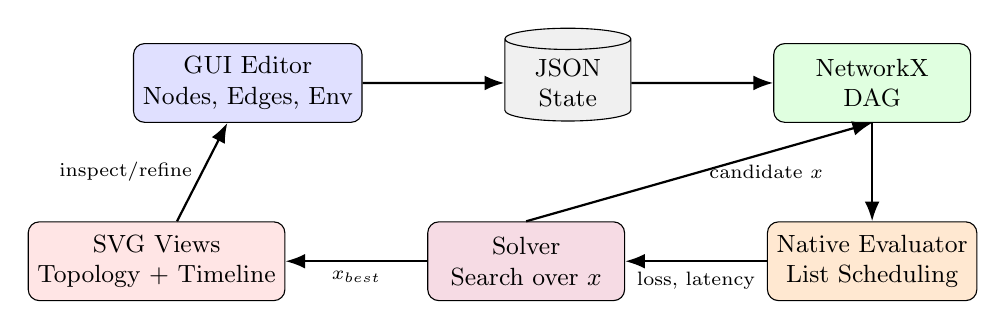
\begin{tikzpicture}[
      block/.style={draw, rounded corners, minimum width=2.5cm, minimum height=1cm, align=center, font=\small},
      arrow/.style={-{Latex[length=2.5mm]}, thick},
      data/.style={draw, cylinder, shape border rotate=90, aspect=0.25, minimum height=1.1cm, minimum width=1.6cm, align=center, font=\small}
    ]
    \node[block, fill=blue!12] (edit) at (0,0) {GUI Editor\\Nodes, Edges, Env};
    \node[data, fill=gray!12, right=1.8cm of edit] (json) {JSON\\State};
    \node[block, fill=green!12, right=1.8cm of json] (graph) {NetworkX\\DAG};
    \node[block, fill=orange!18, below=1.25cm of graph] (eval) {Native Evaluator\\List Scheduling};
    \node[block, fill=purple!14, left=1.8cm of eval] (solver) {Solver\\Search over $x$};
    \node[block, fill=red!10, left=1.8cm of solver] (viz) {SVG Views\\Topology + Timeline};

    \draw[arrow] (edit) -- (json);
    \draw[arrow] (json) -- (graph);
    \draw[arrow] (graph) -- (eval);
    \draw[arrow] (eval) -- node[below, font=\scriptsize] {loss, latency} (solver);
    \draw[arrow] (solver) -- node[below, font=\scriptsize] {$x_{best}$} (viz);
    \draw[arrow] (viz) -- node[left, font=\scriptsize] {inspect/refine} (edit);
    \draw[arrow] (solver.north) -- node[right, font=\scriptsize] {candidate $x$} (graph.south);
  \end{tikzpicture}
  \vspace{0.8em}

  The prototype keeps editing, solving, physical evaluation, and visualization in one reproducible workflow.
\end{frame}

\begin{frame}{Data Model}
  \begin{itemize}
    \item In memory, topology is stored in a \texttt{networkx.DiGraph}.
    \item Node attributes:
      \begin{itemize}
        \item \texttt{id}, \texttt{name}, \texttt{c\_dev}, \texttt{c\_host}, \texttt{fixed\_dev}, \texttt{x}.
        \item Optional input cadence fields: \texttt{source\_period\_ms}, \texttt{source\_phase\_ms}.
      \end{itemize}
    \item Edge attributes:
      \begin{itemize}
        \item \texttt{source}, \texttt{target}, \texttt{size} in MB.
      \end{itemize}
    \item Environment fields:
      \begin{itemize}
        \item \texttt{bandwidth}, \texttt{latency}, \texttt{weight\_avg\_latency}, \texttt{weight\_max\_latency}, \texttt{weight\_device\_utilization}.
        \item \texttt{latency\_limit}, \texttt{max\_frame\_latency\_limit}, \texttt{batch\_transfers}, \texttt{pipeline\_unroll}.
      \end{itemize}
    \item JSON load/save keeps experiments reproducible and shareable.
  \end{itemize}
\end{frame}

\begin{frame}{Queue-Aware Execution}
  \centering
  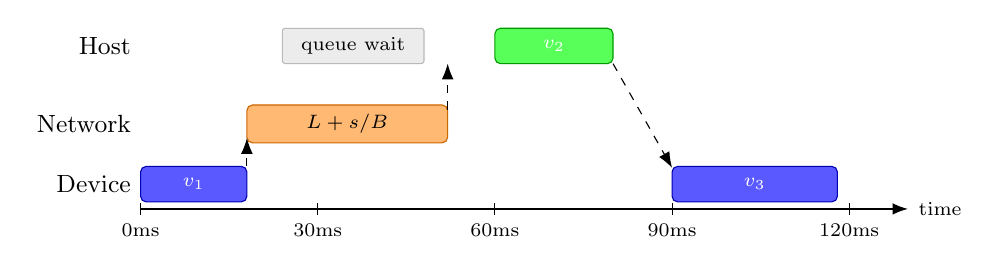
\begin{tikzpicture}[
      x=0.075cm, y=0.9cm,
      axis/.style={-{Latex[length=2mm]}, thick},
      opdev/.style={draw=blue!70!black, fill=blue!65, text=white, rounded corners=2pt, minimum height=0.45cm, font=\scriptsize},
      ophost/.style={draw=green!60!black, fill=green!65, text=white, rounded corners=2pt, minimum height=0.45cm, font=\scriptsize},
      transfer/.style={draw=orange!80!black, fill=orange!55, rounded corners=2pt, minimum height=0.35cm, font=\scriptsize},
      wait/.style={draw=gray!55, fill=gray!15, rounded corners=1pt, minimum height=0.28cm, font=\scriptsize}
    ]
    \draw[axis] (0,0) -- (130,0) node[right] {\scriptsize time};
    \foreach \x/\t in {0/0,30/30,60/60,90/90,120/120}
      \draw (\x,0.08) -- (\x,-0.08) node[below] {\scriptsize \t ms};

    \node[left] at (0,2.3) {\small Host};
    \node[left] at (0,1.2) {\small Network};
    \node[left] at (0,0.35) {\small Device};

    \node[opdev, minimum width=18*0.075cm] at (9,0.35) {$v_1$};
    \node[transfer, minimum width=34*0.075cm] at (35,1.2) {$L+s/B$};
    \node[wait, minimum width=24*0.075cm] at (36,2.3) {queue wait};
    \node[ophost, minimum width=20*0.075cm] at (70,2.3) {$v_2$};
    \node[opdev, minimum width=28*0.075cm] at (104,0.35) {$v_3$};

    \draw[dashed, -{Latex[length=2mm]}] (18,0.6) -- (18,1.0);
    \draw[dashed, -{Latex[length=2mm]}] (52,1.4) -- (52,2.05);
    \draw[dashed, -{Latex[length=2mm]}] (80,2.05) -- (90,0.58);
  \end{tikzpicture}
  \vspace{0.8em}

  A node starts only after all data is ready and its assigned worker queue is available.
\end{frame}

\begin{frame}{Evaluator Step 1: Expanded Task DAG}
  For a candidate assignment $x$, the C++ core expands the unrolled pipeline into a task DAG.
  \begin{itemize}
    \item Source tasks: zero-duration releases at $phase_i+f\cdot period_i$.
    \item Compute tasks: one task per non-source node and frame.
    \item Cross-device edges: explicit Network tasks with cost $L+s/B$.
    \item Batched outgoing transfers: one Network task with $L+\sum_k s_k/B$.
  \end{itemize}
  Dependency classes:
  \begin{itemize}
    \item Same-device data edge: source compute/source task $\rightarrow$ target compute task.
    \item Cross-device data edge: source task $\rightarrow$ Network task $\rightarrow$ target task.
    \item Same non-input operator across frames: FIFO edges from frame $f$ to $f+1$.
  \end{itemize}
\end{frame}

\begin{frame}{Evaluator Step 2: Ready-List Event Loop}
  The simulator maintains pending dependencies, earliest ready times, and one serialized ready time per resource:
  \[
    time\_dev\_ready,\quad time\_host\_ready,\quad time\_network\_ready
  \]
  A ready task starts at:
  \[
    S_t =
    \begin{cases}
      ready_t, & resource(t)=source \\
      \max(ready_t, time\_dev\_ready), & resource(t)=device \\
      \max(ready_t, time\_host\_ready), & resource(t)=host \\
      \max(ready_t, time\_network\_ready), & resource(t)=network
    \end{cases}
  \]
  Main loop:
  \begin{enumerate}
    \item Put zero-pending tasks into the ready set.
    \item Pick the ready task with the earliest feasible start time.
    \item Break ties with the active rule priority.
    \item Record start/finish, update the resource queue, and release successors.
  \end{enumerate}
\end{frame}

\begin{frame}{Evaluator Step 3: Ensemble Rules}
  The task DAG and upward ranks are built once per assignment:
  \[
    rank(t)=duration(t)+\max_{u \in succ(t)} rank(u)
  \]
  The evaluator simulates seven deterministic rules:
  \begin{itemize}
    \item \textbf{CriticalPath}: higher rank first, with older-frame aging
      \[
        rank(t)+10^6\max(0, unroll-1-frame(t)).
      \]
    \item \textbf{DeviceFirst}: source tasks, then Device, then Network, then Host; duration and rank break ties.
    \item \textbf{HostFirst}: source tasks, then Host, then Network, then Device.
    \item \textbf{NetworkFirst}: source tasks, then Network, then Device, then Host.
    \item \textbf{OutputFirst}: output compute tasks first, then older-frame aging and rank.
    \item \textbf{Throughput}: younger-frame aging and rank to test steady-state pipeline schedules.
    \item \textbf{FifoReady}: stable creation order after earliest feasible start time.
  \end{itemize}
  The earliest-start selection keeps the scheduler work-conserving; priorities decide only among tasks that can start at the same time.
\end{frame}

\begin{frame}{Evaluator Step 4: Tail-Latency Retiming}
  The evaluator reduces artificial long tail-frame E2E windows without adding frame-wide gates:
  \begin{itemize}
    \item \textbf{Deferred blocked transfers}: if a cross-device target is still blocked by other prerequisites, delay the transfer until those prerequisites finish.
    \item \textbf{Right-shift sweep}: after list scheduling, move slack network tasks and join-side branch work later, as long as successors, resource order, releases, and output finish times remain unchanged.
  \end{itemize}
  This avoids counting early work that cannot help output completion as the frame's first non-input event, while preserving true inter-frame overlap.
  \vspace{0.5em}

  Per assignment, the native core evaluates:
  \[
    2 \times 2 \times 7 = 28
  \]
  deterministic list schedules: two transfer timings, retiming on/off, and seven ready-list rules.
\end{frame}

\begin{frame}{Evaluator Step 5: Metrics and Winner Selection}
  Latency excludes source/input events.
  For each frame:
  \[
    frame\_start=\min(\text{non-input compute starts, transfer starts})
  \]
  \[
    frame\_finish=\max(\text{non-input output finishes})
  \]
  \[
    \tau_{frame}=frame\_finish-frame\_start
  \]
  Reported metrics:
  \[
    \tau_{max}=\max_f \tau_{frame}(f),\quad
    \tau_{avg}=\frac{pipeline\_finish-pipeline\_start}{pipeline\_unroll}
  \]
  The winner is the schedule with lowest split loss. Ties prefer lower max-frame latency, then lower average latency, then lower initiation interval, then higher Device utilization.
\end{frame}

\begin{frame}{Network Batching Illustration}
  \centering
  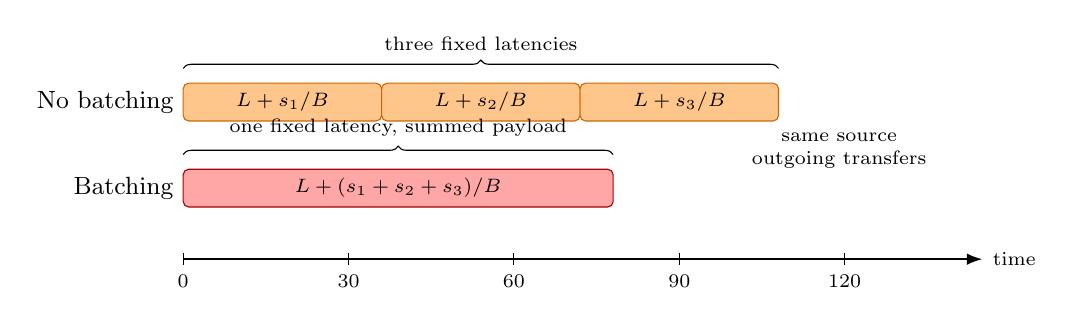
\begin{tikzpicture}[
      x=0.07cm, y=0.95cm,
      axis/.style={-{Latex[length=2mm]}, thick},
      edgebar/.style={draw=orange!80!black, fill=orange!45, rounded corners=2pt, minimum height=0.38cm, font=\scriptsize},
      batchbar/.style={draw=red!65!black, fill=red!35, rounded corners=2pt, minimum height=0.38cm, font=\scriptsize},
      label/.style={font=\small}
    ]
    \draw[axis] (0,0) -- (145,0) node[right] {\scriptsize time};
    \foreach \x/\t in {0/0,30/30,60/60,90/90,120/120}
      \draw (\x,0.08) -- (\x,-0.08) node[below] {\scriptsize \t};

    \node[label, left] at (0,2.1) {No batching};
    \node[edgebar, minimum width=36*0.07cm] at (18,2.1) {$L+s_1/B$};
    \node[edgebar, minimum width=36*0.07cm] at (54,2.1) {$L+s_2/B$};
    \node[edgebar, minimum width=36*0.07cm] at (90,2.1) {$L+s_3/B$};
    \draw[decorate, decoration={brace, amplitude=3pt}] (0,2.55) -- (108,2.55)
      node[midway, above=3pt, font=\scriptsize] {three fixed latencies};

    \node[label, left] at (0,0.95) {Batching};
    \node[batchbar, minimum width=78*0.07cm] at (39,0.95) {$L+(s_1+s_2+s_3)/B$};
    \draw[decorate, decoration={brace, amplitude=3pt}] (0,1.4) -- (78,1.4)
      node[midway, above=3pt, font=\scriptsize] {one fixed latency, summed payload};

    \node[font=\scriptsize, align=center] at (119,1.45) {same source\\outgoing transfers};
  \end{tikzpicture}
  \vspace{0.8em}

  Batching reduces repeated fixed latency, but it does not allow network transfers to overlap.
\end{frame}

\begin{frame}{Network Model: Serialized Transfers and Batching}
  \begin{itemize}
    \item Cross-device transfers share one network worker timeline:
      \[
        time\_network\_ready
      \]
    \item A transfer can start only after its source node finishes and the network worker is idle.
    \item Without batching, each cross-device edge is scheduled independently:
      \[
        T_{edge}=L+\frac{s}{B}
      \]
    \item With \texttt{batch\_transfers=true}, multiple outgoing cross-device edges from the same source node are sent as one transaction:
      \[
        T_{batch}=L+\frac{\sum_k s_k}{B}
      \]
    \item This preserves non-overlap while avoiding repeated fixed latency for successive outgoing transfers.
  \end{itemize}
\end{frame}

\begin{frame}{Objective and Feasibility}
  The solver minimizes a weighted objective:
  \[
    J =
    w_{avg} L_{avg}
    + w_{max} L_{max}
    + w_{util} L_{util}
  \]
  where
  \[
    L_{avg}=\frac{\tau}{\max(scale_{avg}, 1)},\quad
    L_{max}=\frac{\tau_{frame}^{max}}{\max(scale_{max}, 1)},\quad
    L_{util}=1-\frac{device\_active\_time}{pipeline\_work\_span}
  \]
  The latency scales come from all-device/all-host baselines.
  \vspace{0.5em}
  \begin{block}{Latency limits}
    Positive limits act as hard feasibility constraints:
    \[
      \tau \leq latency\_limit,\quad
      \tau_{frame}^{max} \leq max\_frame\_latency\_limit
    \]
    A zero value disables that limit. Candidates above either enabled limit are rejected before objective comparison.
  \end{block}
\end{frame}

\begin{frame}{Solver Modes}
  \begin{table}
    \centering
    \small
    \begin{tabular}{p{0.2\textwidth}p{0.23\textwidth}p{0.46\textwidth}}
      \toprule
      Mode & Use case & Behavior \\
      \midrule
      Auto & Default & Enumerates if $\leq 12$ free nodes; otherwise random search \\
      Enumerate & Small DAGs & Splits assignment masks across threads; returns the exact feasible global best \\
      Random Search & Larger DAGs & Runs independent threaded perturbation chains and keeps the best feasible candidate \\
      Simulated Annealing & Escaping local minima & Runs independent threaded annealing chains with configurable initial/final temperatures \\
      \bottomrule
    \end{tabular}
  \end{table}
  \vspace{0.5em}
  \texttt{solver\_threads}=0 selects the hardware thread count. All modes enforce fixed-device nodes plus the average E2E and max-frame latency caps.
\end{frame}

\begin{frame}{GUI Workflow}
  \begin{enumerate}
    \item Edit nodes, names, compute costs, fixed-device flags.
    \item Edit edges and transfer sizes in MB.
    \item Configure bandwidth, latency, network batching, objective weights, solver mode, threads, iterations, SA temperatures, and latency caps.
    \item Click \textbf{Solve}.
    \item Inspect latency, resource utilization, topology placement, and profiler-style timeline.
  \end{enumerate}
  \vspace{0.5em}
  Validation catches duplicate node IDs, unknown edge endpoints, and non-DAG topologies.
\end{frame}

\begin{frame}{Visualization Design}
  \begin{columns}[T,onlytextwidth]
    \begin{column}{0.5\textwidth}
      \textbf{Topology SVG}
      \begin{itemize}
        \item Config DAG shows transfer size and local/cross-device edge style before solving.
        \item Solved pipeline uses high-contrast node fill color for frame identity.
        \item Blue outline: \device; green outline: \host.
        \item Bold or dashed source styling marks fixed-device and input/source events.
        \item FIFO, transfer, local, and release lines follow the same frame color as the source frame.
      \end{itemize}
    \end{column}
    \begin{column}{0.5\textwidth}
      \textbf{Timeline SVG}
      \begin{itemize}
        \item Input, Host, Transfer, and Device lanes.
        \item Operator bars use computed start/finish times and the same frame fill color as the solved topology.
        \item Transfer bars use actual evaluator records, including serialized and batched transfers.
        \item Input release dots, spans, and vertical release/dependency lines use the matching frame color.
        \item Browser-native scroll and scale controls.
      \end{itemize}
    \end{column}
  \end{columns}
\end{frame}

\begin{frame}{Topology and Timeline Reading Guide}
  \centering
  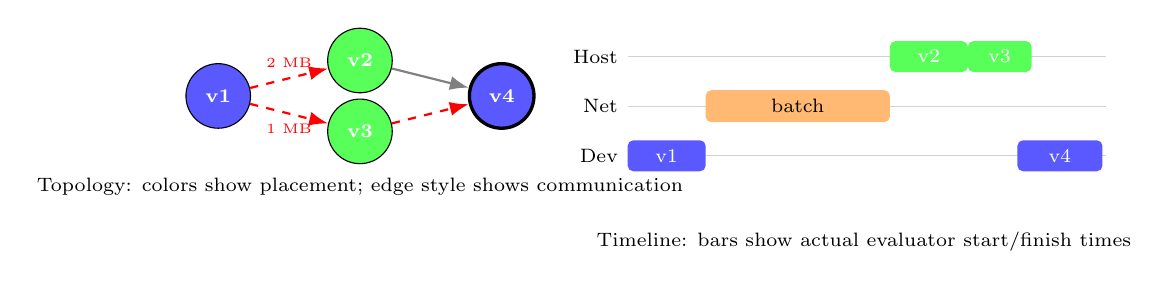
\begin{tikzpicture}[
      node/.style={circle, draw=black, minimum size=0.82cm, font=\bfseries\scriptsize},
      arrow/.style={-{Latex[length=2.4mm]}, thick},
      lane/.style={draw=gray!35},
      op/.style={rounded corners=2pt, minimum height=0.32cm, font=\scriptsize},
      x=1cm, y=1cm
    ]
    \node[node, fill=blue!65, text=white] (a) at (0,2.9) {v1};
    \node[node, fill=green!65, text=white] (b) at (1.8,3.35) {v2};
    \node[node, fill=green!65, text=white] (c) at (1.8,2.45) {v3};
    \node[node, fill=blue!65, text=white, line width=1.2pt] (d) at (3.6,2.9) {v4};
    \draw[arrow, red, dashed] (a) -- node[above, font=\tiny] {2 MB} (b);
    \draw[arrow, red, dashed] (a) -- node[below, font=\tiny] {1 MB} (c);
    \draw[arrow, gray] (b) -- (d);
    \draw[arrow, red, dashed] (c) -- (d);
    \node[font=\scriptsize] at (1.8,1.75) {Topology: colors show placement; edge style shows communication};

    \begin{scope}[shift={(5.2,2.0)}, x=0.045cm, y=0.7cm]
      \draw[lane] (0,2.0) -- (135,2.0);
      \draw[lane] (0,1.1) -- (135,1.1);
      \draw[lane] (0,0.2) -- (135,0.2);
      \node[left, font=\scriptsize] at (0,2.0) {Host};
      \node[left, font=\scriptsize] at (0,1.1) {Net};
      \node[left, font=\scriptsize] at (0,0.2) {Dev};
      \node[op, fill=blue!65, text=white, minimum width=22*0.045cm] at (11,0.2) {v1};
      \node[op, fill=orange!55, minimum width=52*0.045cm] at (48,1.1) {batch};
      \node[op, fill=green!65, text=white, minimum width=22*0.045cm] at (85,2.0) {v2};
      \node[op, fill=green!65, text=white, minimum width=18*0.045cm] at (105,2.0) {v3};
      \node[op, fill=blue!65, text=white, minimum width=24*0.045cm] at (122,0.2) {v4};
    \end{scope}
    \node[font=\scriptsize] at (8.2,1.05) {Timeline: bars show actual evaluator start/finish times};
  \end{tikzpicture}
\end{frame}

\begin{frame}{Example DAG}
  \centering
  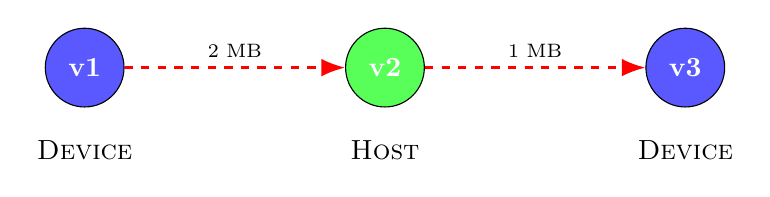
\begin{tikzpicture}[
      node/.style={circle, draw=black, minimum size=1cm, font=\bfseries},
      edge/.style={-{Latex[length=3mm]}, thick},
      local/.style={edge, draw=gray},
      remote/.style={edge, draw=red, dashed}
    ]
    \node[node, fill=blue!65, text=white] (v1) {v1};
    \node[node, fill=green!65, text=white, right=2.8cm of v1] (v2) {v2};
    \node[node, fill=blue!65, text=white, right=2.8cm of v2] (v3) {v3};
    \draw[remote] (v1) -- node[above, font=\scriptsize] {2 MB} (v2);
    \draw[remote] (v2) -- node[above, font=\scriptsize] {1 MB} (v3);
    \node[below=0.3cm of v1] {\device};
    \node[below=0.3cm of v2] {\host};
    \node[below=0.3cm of v3] {\device};
  \end{tikzpicture}
  \vspace{1em}

  The evaluator produces a queue-aware schedule rather than an ideal infinite-parallel critical path.
\end{frame}

\begin{frame}{Current Implementation Stack}
  \begin{itemize}
    \item Python 3.9+.
    \item PyQt6 for desktop controls and layout.
    \item PyQt6-WebEngine for SVG topology and timeline rendering.
    \item NetworkX for DAG storage, topological sort, and validation.
    \item C++/pybind11 native core for schedule evaluation, objective scoring, and solver search.
    \item Pytest coverage for evaluator, JSON IO, solver modes, and latency-limit feasibility.
    \item Launch commands: \texttt{python -m coopinfer} or \texttt{python -m coopinfer.app}.
  \end{itemize}
\end{frame}

\begin{frame}{Next Steps}
  \begin{itemize}
    \item Add richer solver diagnostics: rejected candidates, constraint slack, convergence history.
    \item Add exportable SVG/PNG reports for topology and timeline.
    \item Add batch evaluation over bandwidth/latency sweeps.
    \item Expose selected scheduling rule, queue slack, and ready-task diagnostics.
    \item Improve timeline semantics with explicit queue-wait and data-ready intervals.
    \item Explore additional network reordering policies and transfer-priority rules.
  \end{itemize}
\end{frame}

\begin{frame}
  \centering
  \Huge Questions?
\end{frame}

\end{document}
